
%%%%%%%% HZZ4l %%%%%%%
%%%>  Introduction <%%%

\section{Introduction}
\label{sec:introduction}

The standard model (SM) of electroweak interactions~\cite{StandardModel67_1,StandardModel67_2,StandardModel67_3}
relies on the existence of the Higgs boson, $\PH$, a scalar particle associated with the field responsible for
spontaneous electroweak symmetry breaking~\cite{Englert:1964et,Higgs:1964ia,Higgs:1964pj,Guralnik:1964eu,Higgs:1966ev,Kibble:1967sv}.
The mass of the boson, $\mH$, is not fixed by the theory. Previous searches at LEP and the Tevatron 
excluded at 95\% confidence level (CL) masses lower than $114.4~\GeV$~\cite{Barate:2003sz} and the mass range $162-166~\GeV$~\cite{TEVHIGGS_2010}, respectively. Previous direct searches at the Large Hadron Collider (LHC)~\cite{Evans:2008zzb} were based on data from proton-proton (pp) collisions corresponding to 
an integrated luminosity of around 5\fbinv, collected at a center-of-mass energy $\sqrt{s}=7\TeV$.
The CMS experiment has excluded at 95\% CL masses from 127 to 600\,GeV~\cite{Chatrchyan:2012tx}. The ATLAS experiment excluded at 95\% CL the ranges 111.4--116.4, 119.4--122.1 and 129.2--541\unit{GeV}~\cite{ATLAS:2012ae, atlas:20127tev}.
In 2012, the LHC pp center-of-mass energy was increased to $\sqrt{s}=8\TeV$, and an additional integrated luminosity
of more than 5\fbinv was recorded by the end of June by each of these experiments. Searches based on these data in the mass range 110--145\GeV led to the
observation of a new boson, consistent with the SM Higgs boson, with a mass of approximately 
$125\GeV$~\cite{CMSobservation125,ATLASobservation125}.
The analysis presented in this paper extends these searches to
a high mass region 145--1000\GeV.

%% ED: I think some of comments below are quite good in terms of motivation - perhaps one or two sentences, justifying the high mass searches, should go back in?


%{\it removed
%Given the fact that an overall excess is found at the low end of the 
%mass spectrum explored by
%both the LHC and Tevatron experiments, the main interest in the Higgs 
%searches is currently
%focused on that mass region.
%Moreover there are classic upper bounds on the Higgs-boson mass coming 
%from 
%unitarity~\cite{Veltman:1976rt,Lee:1977yc,Lee:1977eg,Passarino:1990hk}, 
%triviality and
%vacuum stability, precision electroweak data and absence of fine-tuning (for a
%recent review see Ref.~\cite{Ellis:2009tp}).
%Nevertheless, in view of the role of the Higgs boson in the unitarization of 
%the diboson-scattering at high energy,
%it is of primary importance to keep studying the high mass region,
%in particular processes which involve the vector-boson fusion (VBF) 
%production mechanism.
%
%It has been proposed that the low mass boson can be interpreted as 
%imposter~\cite{Low:2011gn,Low:2012rj}
%with no connection with the electroweak symmetry breaking mechanism. In this
%interpretation, the SM Higgs boson has still to be searched for. On the 
%other hand, 
%%given the compelling role of the
%%Higgs in the unitarization of the theory, 
%many BSM models, which predict 
%the presence of additional resonances
%at high mass (Higgs mass splitting), can be built as
%modification of the SM case. In all these models, theoretical issues 
%related with the width of the resonance
%and the interference with the background, will have to be addressed. A 
%correct treatment of these
%problems needs to be established first in the SM case.
%%, as will be shown 
%%in the following.
%}

The Higgs mechanism plays an important role in the unitarization of diboson scattering at high 
energies~\cite{Dicus:1992vj,Veltman:1976rt,Lee:1977eg,Lee:1977yc,Passarino:1990hk,Chanowitz:1985hj,Duncan:1985vj,Dicus:1986jg,Bagger:1995mk,Ballestrero:2009vw}. 
The newly-discovered boson could be interpreted as an 'imposter'~\cite{Low:2011gn,Low:2012rj}, with no connection with the electroweak symmetry breaking mechanism.
In addition, several popular scenarios, such as general two Higgs doublet models (for a review see~\cite{Branco:2011iw}) or models
in which the SM Higgs boson mixes with a heavy electroweak singlet~\cite{Patt:2006fw}, predict the existence
of an additional resonance at high mass, with couplings similar to the SM Higgs boson. In any such models, theoretical 
issues related to the width of the resonance and its interference with background must be understood. A correct treatment
of these problems needs to be established first in the SM case. This paper therefore reports a search for a Higgs boson at 
high mass, assuming the properties predicted by the SM. The $\PH \to \WW$ and $\PH \to \ZZ$ decay channels are used as 
benchmarks for cross section and production mechanism in the mass range $145 < \mH < 1000$ GeV. This approach allows a 
self-consistent and coherent presentation of the results of high mass searches, paving the way for future model-independent 
searches for BSM heavy resonances.

%% ED: Missing citations above

%% ED: Do we actually mean model-independent here?

For $\mH \ge 2\mW$, the main discovery channels at the LHC are those with two real weak bosons: $\WW$ for
$2\mW \le \mH < 2 \mZ$, and in addition $\ZZ$ for $\mH \ge 2\mZ$. 
For a Higgs boson decaying to two $\PW$ bosons, the
fully leptonic ($\PH \to \WW \to \ell\nu\ell\nu$) and semileptonic ($\PH \to \WW \to \ell \nu
\mathrm{qq}$) final states are considered in this analysis. For a Higgs boson decaying into two $\cPZ$
bosons, final states containing four leptons ($\PH \to \ZZ \to 2\ell 2\ell '$), two leptons and two
jets ($\PH \to \ZZ \to 2\ell \mathrm{qq}$), and two leptons and two neutrinos
($\PH \to \ZZ \to 2\ell 2\nu$), are considered, where $\ell = \Pe$ or $\Pgm$ and $\ell ' = \Pe$, $\Pgm$
or $\Pgt$. The analyses use pp collision data samples recorded by the CMS detector, corresponding to integrated
luminosities of up to 5.1 ${\rm fb}^{-1}$ at $\sqrt{s} = 7\TeV$ and up to 5.3 ${\rm fb}^{-1}$ at
$\sqrt{s} = 8\TeV$.

\section{CMS detector and simulations}
\label{sec:cms}

CMS uses a right-handed coordinate system, with the origin at the nominal interaction point, the $x$ axis
pointing to the center of the LHC ring, the $y$ axis pointing up (perpendicular to the plane of the LHC ring),
and the $z$ axis along the counterclockwise-beam direction. The polar angle $\theta$ is measured from the
positive $z$ axis, and the azimuthal angle $\phi$ is measured in the $x$--$y$ plane. The pseudorapidity
is defined as $\eta=-{\rm ln}[\tan{(\theta/2)}]$. The magnitude of the transverse momentum ($\PT$) is calculated as $\PT = \sqrt{p_x^2 + p_y^2}$. Missing transverse energy $\met$ is defined as the modulus of the negative vector sum of the transverse momenta of all reconstructed particles,
charged and neutral, in an event.

The central feature of the CMS apparatus is a superconducting solenoid of 6\unit{m} internal diameter, which
provides a magnetic field of 3.8\unit{T}. Within the field volume are a silicon pixel and strip tracker,
a lead tungstate crystal electromagnetic calorimeter (ECAL), and a brass/scintillator hadron calorimeter
(HCAL). A quartz-fiber Cherenkov calorimeter extends the coverage to $|\eta| < 5.0$. Muons are measured in
gas-ionization detectors embedded in the steel flux-return yoke. The first level of the CMS trigger system, composed of custom hardware processors, is designed to select the most interesting events in less than $3\mu$s, using information from the calorimeters and muon detectors. The High Level Trigger processor farm decreases the event rate from 100 kHz delivered by the first level trigger to a few hundred Hz, before data storage. A full description of the CMS apparatus is
available elsewhere~\cite{Chatrchyan:2008zzk}.

Several Monte Carlo (MC) event generators are used to simulate the signals and backgrounds. 
The $\PH \rightarrow \WW(\ZZ)$ signal is simulated using the next-to-leading order (NLO) package
{\sc powheg}~\cite{Alioli:2008gx,Nason:2004rx,Frixione:2007vw}. The Higgs boson signals from gluon fusion ($\Pg\Pg \rightarrow \PH$),
and vector-boson fusion (VBF, $\Pq\Pq \rightarrow \Pq\Pq \PH$), are generated with {\sc powheg} at NLO and a dedicated
program~\cite{Gao:2010qx} used for angular correlations. Samples of $\PW\PH$, $\cPZ\PH$, and $\ttbar\PH$ events are
generated using \PYTHIA 6.424~\cite{Sjostrand:2006za}.

%% ED: Angular correlations of the decay products, right? Should clarify.

Events at generator level are weighted according to the total cross section $\sigma(\Pp\Pp\rightarrow \PH)$,
which contains contributions from gluon fusion computed to next-to-next-to-leading order (NNLO) and next-to-next-to-leading log~\cite{Anastasiou:2008tj,deFlorian:2009hc,Baglio:2010ae,LHCHiggsCrossSectionWorkingGroup:2011ti,Djouadi:1991tka,Dawson:1990zj,Spira:1995rr,Harlander:2002wh,Anastasiou:2002yz,Ravindran:2003um,Catani:2003zt,Actis:2008ug}, and from
weak-boson fusion computed at NNLO~\cite{LHCHiggsCrossSectionWorkingGroup:2011ti,Ciccolini:2007jr,Ciccolini:2007ec,Figy:2003nv,Arnold:2008rz,Bolzoni:2010xr}.
%The total cross section is scaled by the branching fractions calculated
%with \textsc{prophecy4f}, which includes NLO QCD and electroweak corrections and
%all interference effects at NLO~\cite{LHCHiggsCrossSectionWorkingGroup:2011ti,Bredenstein:2006rh,Bredenstein:2006ha,hdecay2,Actis:2008ts}, in particular effects specific to the $4\Pe$ and $4\Pgm$
%channels.

\begin{figure}[htbp]
\centering
   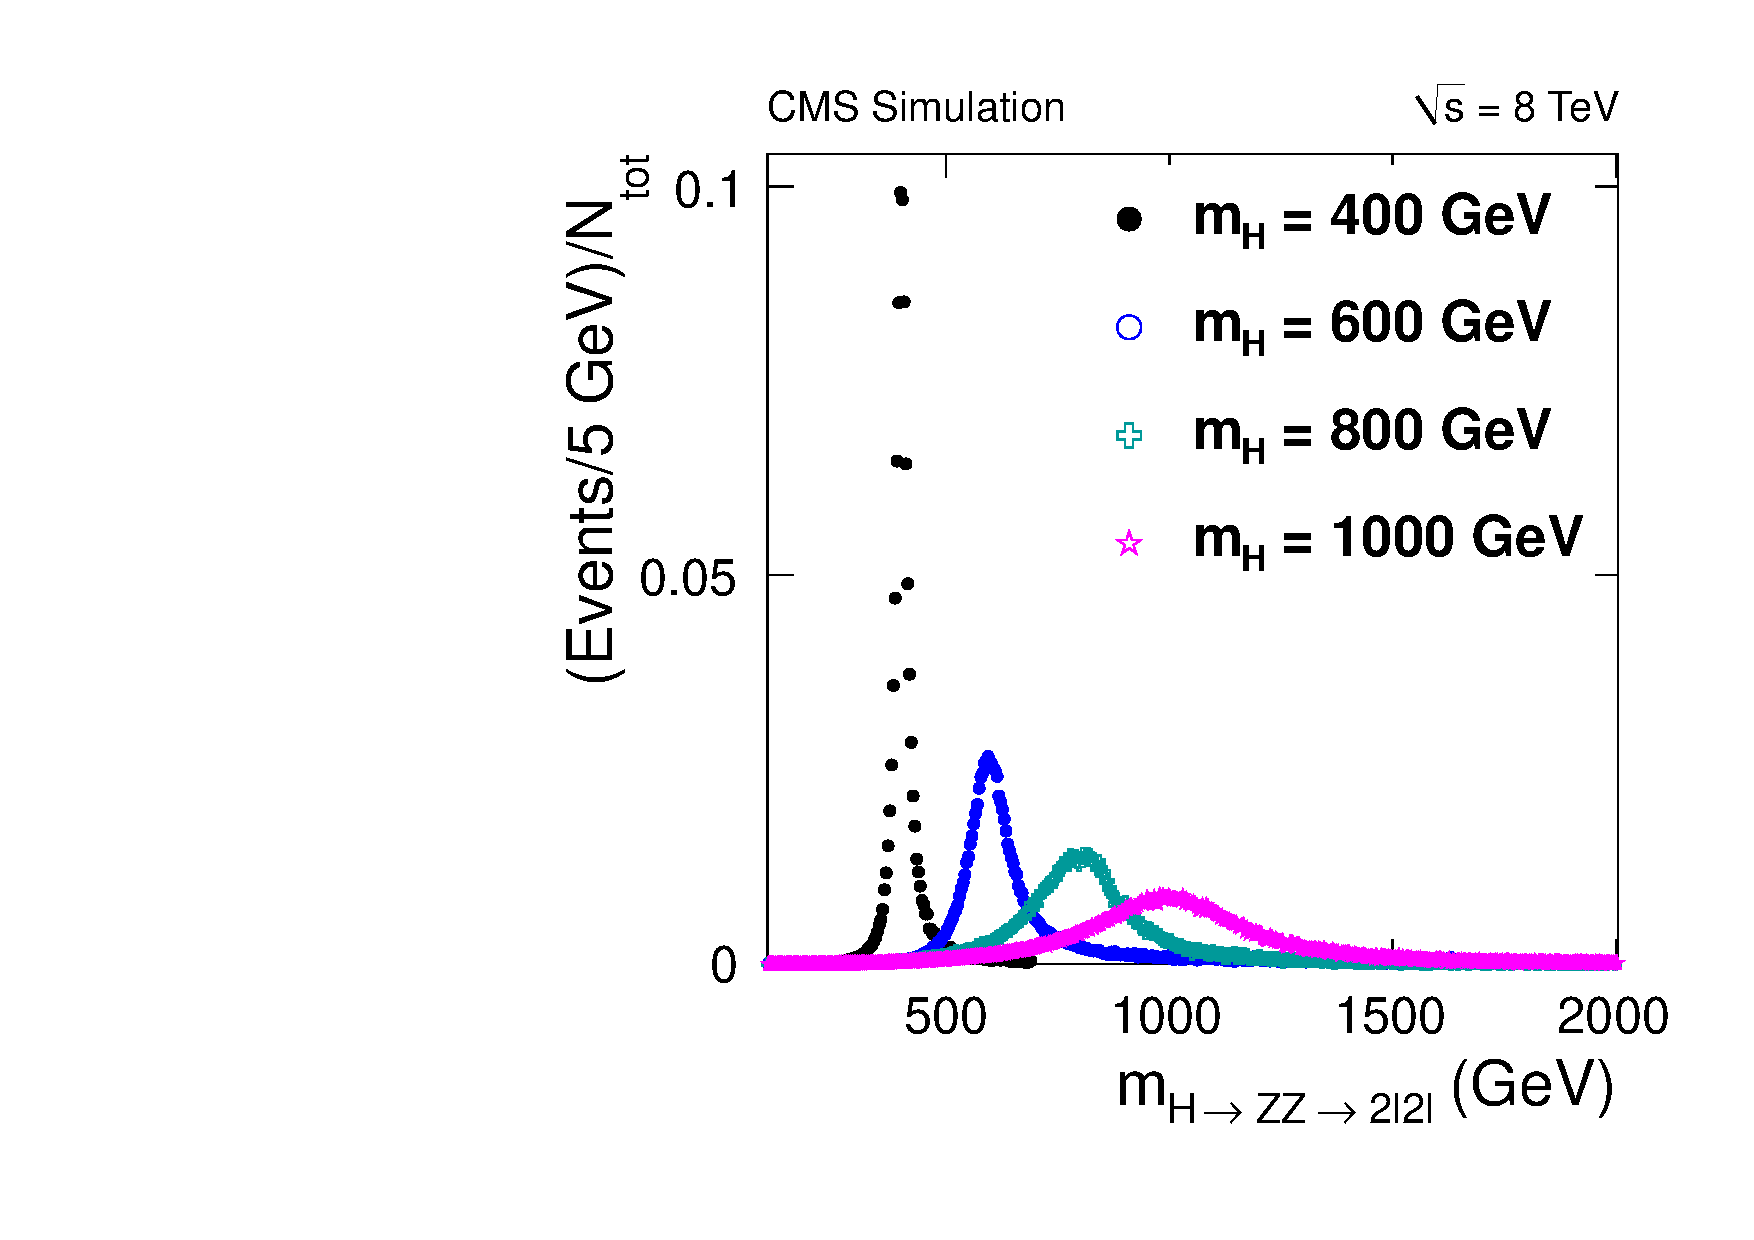
\includegraphics[width=0.6\textwidth]{figures/HiggsMasses.pdf}
   \caption{Simulated distributions of $m_{\rm{H}}$, for several mass hypotheses, 
    after corrections explained in the text. The area of each distribution is normalized to unity.
   }
\label{fig:higgsmasses}
\end{figure}

The simulated \WW(\ZZ) invariant mass ($m_{\WW(\ZZ)}$) lineshape is corrected to match the results
presented in References~\cite{Passarino:2010qk,Goria:2011wa,Kauer:2012hd}, where the complex-pole scheme
(CPS) for the Higgs propagator is used. The resulting simulated lineshapes for the channel $\PH \to \ZZ
\to 2\ell 2\ell$ are shown in Figure~\ref{fig:higgsmasses}. In the gluon-gluon fusion production channel,
the effects on the lineshape due to interference between Higgs boson signal and the  $\mathrm{gg} \to \WW(\ZZ)$
background are included~\cite{Passarino:2012ri}. The theoretical uncertainties on the lineshape due to missing
higher-order corrections in the interference between background and signal are included in the total uncertainities, in addition to uncertainties
associated with electroweak corrections~\cite{Goria:2011wa,Passarino:2012ri}. Interference outside the Higgs mass
peak has sizable effects on the normalization for those final states where the Higgs invariant mass cannot be fully reconstructed. A correction is applied, taking into account the corresponding theoretical uncertainties, 
in the $\WW \to \ell \nu \rm{qq}$ final state~\cite{Passarino:2012ri}. In the $\WW \to \ell\nu\ell\nu$ and
$\ZZ \to \ell \ell \nu\nu$ final states, the effect of interference on the normalization, as computed in ~\cite{Campbell:2011cu,Kauer:2012ma,MaltoniInPrep}, is included with an associated 100\% uncertainty.
%The effect of interference
%in the VBF production is still under study.

% ED: If the above commented text stands, should this not be clarified in the text?

The background contribution from $\rm{q\bar{q}} \to \WW$ production is generated using the \MADGRAPH package~\cite{Alwall:2007st}, and the subdominant $\mathrm{gg} \to \WW$ process is generated using {\tt gg2ww}~\cite{ggww}.
The $\rm{q\bar{q}} \to \ZZ$ production process is simulated at NLO 
with \POWHEG, and the $\rm{gg} \to \ZZ$ process is simulated using
{\tt gg2zz}~\cite{Binoth:2008pr}. Other diboson processes ($\PW\cPZ$, $\cPZ\gamma$, $\PW\gamma^{(*)}$) are generated with \PYTHIA6.424 and \MADGRAPH. The $\cPZ$+jet samples are generated with \MADGRAPH. The $\ttbar$ and $\tw$ events are generated at NLO with \POWHEG.
For leading-order (LO) generators, the default set of parton distribution functions (PDF) used to produce these samples is CTEQ6L~\cite{CTEQ66}, while CT10~\cite{ct10} is used for NLO generators. Tau decays are generated with \textsc{TAUOLA}~\cite{Jadach:1993hs}. The detector response is simulated using a detailed description of the CMS detector, based on the \GEANTfour package~\cite{GEANT}, and event reconstruction is performed identically to that for recorded data.
The simulated samples are reweighted in order to correctly reproduce the distribution of pp interactions per bunch crossing (pileup) as measured in the data.

%% ED: Missing / repeated citations above

\section{Event reconstruction}
\label{sec:reconstruction}

A complete reconstruction of the individual particles emerging from each collision event is obtained via a particle-flow (PF) technique~\cite{CMS-PAS-PFT-09-001, CMS-PAS-PFT-10-002}. This approach uses the information from all CMS sub-detectors to identify and reconstruct individual particles in the collision event, classifying them into mutually exclusive categories: charged hadrons, neutral hadrons, photons, electrons, and muons.

The electron reconstruction algorithm combines information from clusters of energy deposits in the ECAL with the
trajectory in the inner tracker~\cite{Baffioni:2006cd,CMS-PAS-EGM-10-004}. Trajectories in the tracker volume are reconstructed using a dedicated model of electron energy loss, and fitted with a Gaussian sum filter. Electron identification relies on a multivariate technique that combines observables sensitive to the amount of bremsstrahlung
along the electron trajectory, the geometrical and momentum matching between the electron trajectory and
the associated clusters, and shower-shape observables.

The muon reconstruction algorithm combines information from the silicon tracker and the muon spectrometer. Muons are
selected from amongst the reconstructed muon-track candidates by applying requirements on the track components in
the muon system and on matched energy deposits in the calorimeters~\cite{CMS-PAS-PFT-10-003}.

Tau leptons are identified in both their leptonic decay modes, with an electron or muon as measurable decay
product, and in the hadronic mode (denoted $\tauh$). PF particles are used to reconstruct $\tauh$ using the
'hadron-plus-strip' (HPS) algorithm~\cite{Chatrchyan:2011xq}.

%% ED: Possibly the part on muon reconstruction conveys no new information to the uneducated reader...

Jets are reconstructed from PF candidates by using the anti-$\mathrm{k_{T}}$ clustering algorithm
\cite{Cacciari:2008gp,fastjetmanual} with distance parameter $R = 0.5$. Jet energy corrections are applied to
account for the non-linear response of the calorimeters to the particle energies, and other
instrumental effects. These corrections are based on in-situ calibration using dijet and $\gamma+{\rm jet}$ data
samples~\cite{Chatrchyan:2011ds}. The median energy density due to pileup is evaluated in each event, and the
corresponding energy is subtracted from each jet~\cite{Cacciari:2008gn}. Jets are required to originate at the primary vertex, where the primary vertex is identified as the vertex with the highest summed $\PT^2$ of its associated tracks. 
Jets displaced from the primary vertex in the transverse direction can be tagged as $b$-jets~\cite{CMS-PAS-BTV-11-003}.

%% ED: I added a b-tagging reference back in here.

Charged leptons from $\PW$ and $\cPZ$ boson decays are typically expected to be isolated from other activity in the
event. The isolation of $\Pe$ or $\Pgm$ leptons is therefore ensured by applying requirements on the sum of the 
transverse energies of all reconstructed particles, charged or neutral, within a cone of
$\Delta R = \sqrt{(\Delta \eta)^{2}
+ (\Delta \phi)^{2}} < 0.4$ around the lepton direction, after subtracting the average pileup energy 
estimated using a 'jet area' technique~\cite{Cacciari:2007fd} on an event-by-event basis.

At trigger level, depending on the decay channel, events are required to have a pair of electrons or muons,
one lepton with $\PT > 17\GeV$ and the other with $\PT > 8\GeV$, or a single electron (muon) with $\PT > 27~(24)\GeV$.

%% ED: Is this statement consistent with everything in Section 4? This is not obvious.

The overall efficiencies for trigger selection, reconstruction, identification, and isolation of $\Pe$ and $\Pgm$
are measured from recorded data, using a tag-and-probe technique~\cite{CMS:2011aa} based on an inclusive sample of
$\cPZ$ events. These measurements are performed in several bins of $\PT^{\ell} $ and $ |\eta^{\ell}| $. The
efficiencies for selecting electrons in the ECAL barrel (endcaps) varies from around 
%71\% (65\%) for
%$7 < \PT^{\Pe} < 10\GeV$ to 
82\% (73\%) at $\PT^{\Pe} \simeq 10\GeV$
%, and reaches 
to 90\% (89\%) for
$\PT^{\Pe} \simeq 20\GeV$. It drops to about 85\% in the transition region, $1.44 < |\eta^{\Pe}| <
1.57$, between the ECAL barrel and endcaps. Muons are reconstructed and identified with efficiencies greater than
${\sim}98\%$ in the full $|\eta^{\Pgm}| < 2.4$ range. The efficiency of the $\tau$ identification is around 50\% for
$\pt^\Pgt > 20\GeV$~\cite{Chatrchyan:2011xq}. The overall trigger efficiency 
for events selected for this analysis 
% decay channels considered in this paper 
ranges from 96\% to 99\%.

\section{Data analysis}
\label{sec:analyses}

The final results presented in this paper are obtained by combining Higgs bosons searches exploiting different production and decay modes. A summary of these searches is given in Table~\ref{tab:channels}. The following notation is used in
the summary, and throughout this paper: $(jj)_{VBF}$ refers to dijet pair consistent with the VBF topology, and $(jj)_{\PW(\cPZ)}$ to a dijet pair with an invariant mass consistent with coming from a $\PW(\cPZ)$ dijet decay. The results of these searches in the mass range $\mH < 145\GeV$ are presented in~\cite{CMSobservation125}. In each case, all final states are exclusive, with no overlap between channels. The presence of a signal in any one of the channels, at a certain value of the Higgs boson mass, is expected to manifest itself as an excess extending around that value for a range corresponding to the Higgs boson width convoluted with the $\mH$ resolution. It should be noted that the presence of the boson with $\mH = 125\GeV$ effectively constitutes additional background to the high-mass search in the lower part of the explored mass range. This is not explicitly taken account of, and could potentially lead to an overestimation of an excess in the data, and conservative exclusion limits in channels with poor mass resolution.

%% ED: I have removed the words 'or an upward fluctuation of the background' above. To me, this does not seem to add to the clarity of the paper, but if there some significance I have missed, it should go back in.

%% ED: I wonder if the last sentence ought to be clarified further. An obvious question is 'if not, why not'?

\begin{table}[htbp]
\begin{center}
\small
\caption{Summary information on the analyses included in this paper. The column "\PH prod" indicates the production mechanism targeted by an analysis; it does not imply 100\% purity. The main contribution in the untagged and inclusive categories is always gluon-gluon fusion. For the $\PW\PW \to \ell\nu\ell\nu$ and
$\cPZ\cPZ \to 2\ell 2\ell'$ channels the full possible mass range is shown, but in this paper
both analyses are restricted to the masses above 145\GeV. The 
$\cPZ\cPZ \to 2\ell 2q$ analysis uses only $7\TeV$ data set.
}
\label{tab:channels}
\begin{tabular}{|l|c|l| ccc|}
\hline
\PH & \PH & Exclusive  & No. of & $m_{\PH}$ range  & $m_{\PH}$  \\
 decay & prod  &  final states & channels  & (\GeV)  & resolution \\
\hline\hline
%--------------------------------------------------------------------------------------------------------------------------------------------------------------------------------------------------------------------------------------------------
$\PW\PW \to \ell\nu\ell\nu$      & 0/1-jets  &  (($\Pe\Pe$, $\Pgm\Pgm$), $\Pe\Pgm$) + (0 or 1 jets) &  4         & 110--600         & 20\%  \\ 
$\PW\PW \to \ell\nu\ell\nu$      & VBF-tag    &  $ (($\Pe\Pe$, $\Pgm\Pgm$), $\Pe\Pgm$) + (jj)_{VBF}$  &  2    & 110--600         & 20\%  \\ 
$\PW\PW \to \ell\nu qq$          & untagged  &  $(\Pe\nu, \, \Pgm\nu) + $($(jj)_{\PW}$ with 0 or 1 jets) & 4    & 180--600         & 5--15\%  \\ 
\hline%--------------------------------------------------------------------------------------------------------------------------------------------------------------------------------------------------------------------------------------------------
$\cPZ\cPZ \to 2\ell 2\ell'$             & inclusive  &  $4\Pe, \, 4\Pgm, \, 2\Pe2\Pgm$                                                                          & 3         & 110--1000         & 1-2\%   \\  
      &   &  $(\Pe\Pe, \, \Pgm\Pgm) + (\Pgt\Pgt)$                        & 8         & 200--1000         & 10-15\%  \\  
$\cPZ\cPZ \to 2\ell 2q$          & inclusive  &  $(\Pe\Pe,\Pgm\Pgm) + $($(jj)_{\cPZ}$ with 0, 1, 2 b-tags)                                           & 6         & 200--600 & 3\% \\ 
$\cPZ\cPZ \to 2\ell 2\nu$        & untagged  &  $(\Pe\Pe,\Pgm\Pgm)$ + MET + 0, 1, 2 non-VBF jets                                        & 6       & 200--1000         & 7\%   \\
$\cPZ\cPZ \to 2\ell 2\nu$        & VBF-tag    &  $(\Pe\Pe,\Pgm\Pgm)$ + MET + $(jj)_{VBF}$                                                           & 2         & 200--1000         & 7\%   \\
\hline%--------------------------------------------------------------------------------------------------------------------------------------------------------------------------------------------------------------------------------------------------
\end{tabular}
\end{center}
\end{table}

%% ED: I would add to the table (if physically possible) the BR for each channel and the datasets used.

The results of all analyses are finally combined following the prescription developed by the ATLAS and CMS Collaborations
in the context of the LHC Higgs Combination Group~\cite{LHC-HCG-Report, Chatrchyan:2012tx}, taking into account the systematic uncertainties and their correlations.

